
%%%%%%%%%%%%%%%%%%%%%%%%%%%%%%%%%%%%%%%%%%%%%%%%%%%%%%%%%%%
\section{Object manipulation with hardware robots}\label{sec:realExperiment}
%%%%%%%%%%%%%%%%%%%%%%%%%%%%%%%%%%%%%%%%%%%%%%%%%%%%%%%%%%%
Our experiments use centimeter-scale hardware systems called \emph{kilobots}.  While those are far larger than the micro scale devices we model, using kilobots allows us to emulate a variety of dynamics, while enabling a high degree of control over robot function, the environment, and data collection. The kilobot, reported in \cite{Rubenstein2012,rubenstein2014programmable}, is a low-cost robot designed for testing collective algorithms with large numbers of robots. It is available commercially or as an open source platform from \cite{K-Team2015}.  Each robot is approximately 3 cm in diameter, 3 cm tall, and uses two vibration motors to move on a flat surface at speeds up to 1 cm/s.  Each robot has one ambient light sensor that is used to implement \emph{phototaxis},  moving towards a light source. 

  
\subsection{Environmental setup}  
In these experiments as shown in Fig.~\ref{fig:setup}, we used $n$=100 kilobots, a 1.5 m$\times$1.2 m whiteboard as the workspace, and lights: four 50W LED floodlights  at the corners and four 30W LED floodlights on the sides of a 6 m square centered on the workspace and 1.5 m above the table. An Arduino Uno connected to an 8 relay shield controlled the lights.  

Above the table, an overhead machine vision system tracks the swarm. The vision system identifies obstacles by color segmentation, determines the corners  (used to decrease  variance)  by topology, the object by color segmentation, and identifies robots using color segmentation and circle detection with a circular Hough transform.

The Laser-cut patterns for the neon green fiducial markers on the robots and {\sc Matlab} tracking code are available at our github repository,~\cite{Shahrokhi2015GitHubShapeControl}. 
The objects were 3D printed from ABS plastic with a paper overlay. 
Shapes included a 325 cm$^2$ equilateral triangle, 
%Small Equilateral Triangle 140 cm$^2$,
 324 cm$^2$ square,
 281 cm$^2$ hexagon,
254 cm$^2$ circle, 
and a 486 cm$^2$ (18 cm$\times$27 cm)  rectangle, all shown in Fig.~\ref{fig:setup}.

%\begin{figure*}
%\begin{center}
%	%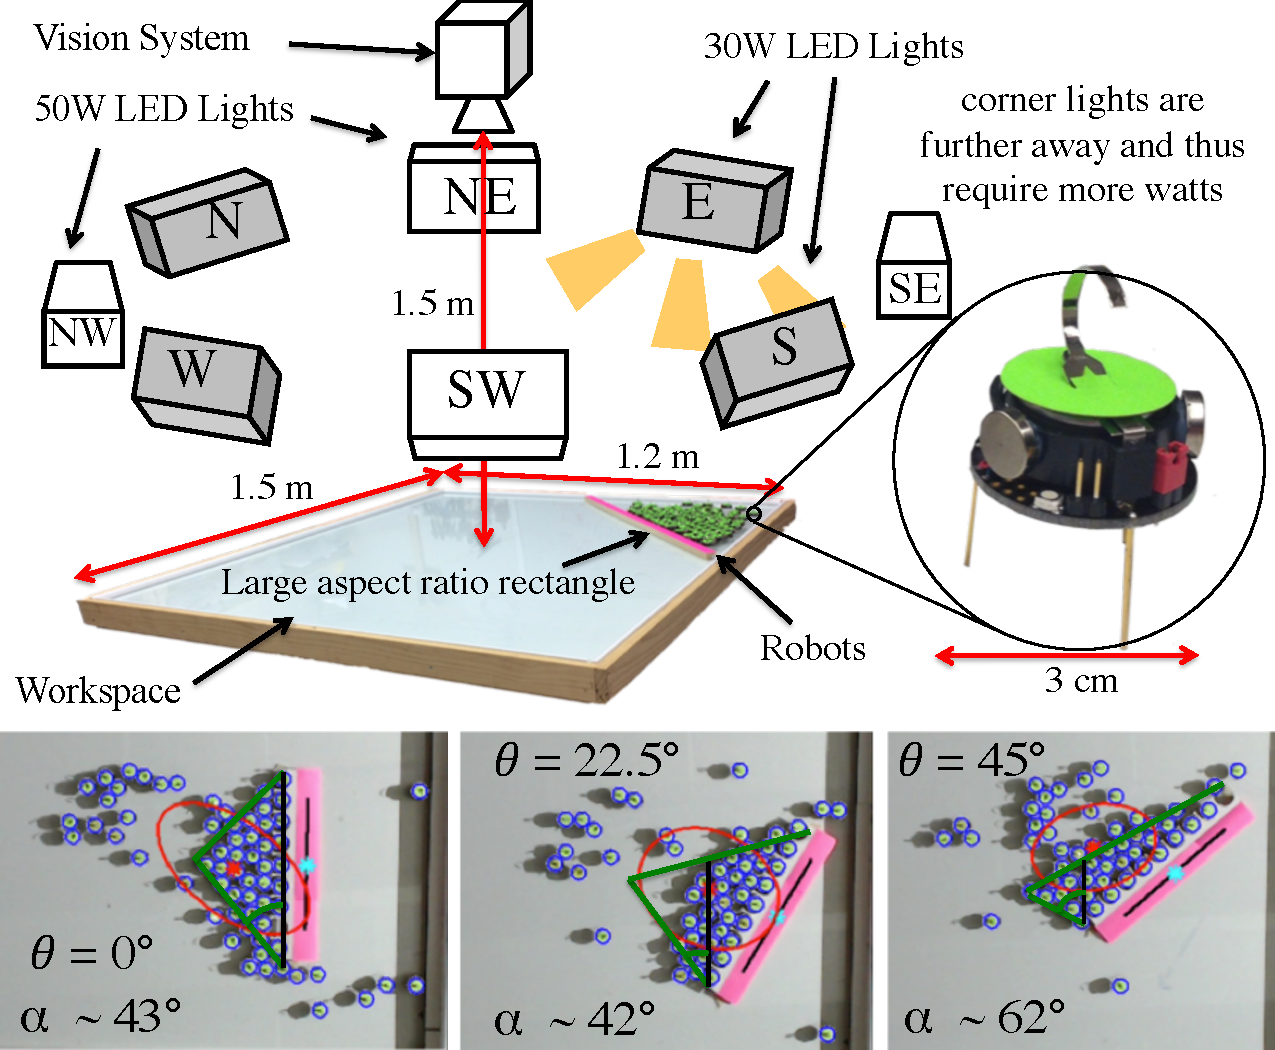
\includegraphics[width=0.5\columnwidth]{SetUp.pdf}
%	\begin{overpic}[width=0.6\columnwidth]{SetUp.pdf}%\put(1,75){A}
%	\end{overpic}\\
%	\begin{overpic}[width=0.35\columnwidth]{AllShapesR.pdf}%\put(-0,85){B}
%	\end{overpic}
%	\begin{overpic}[width=0.35\columnwidth]{PotentialExp.pdf}%\put(-0,85){C}
%	\end{overpic}
%\end{center}
%\caption{\label{fig:setup}
%(Top) Hardware platform. (Lower left) Four shapes used for hardware experiments. (Lower right) Visualization of potential field. }
%\end{figure*}

\begin{figure*}
\begin{center}
	%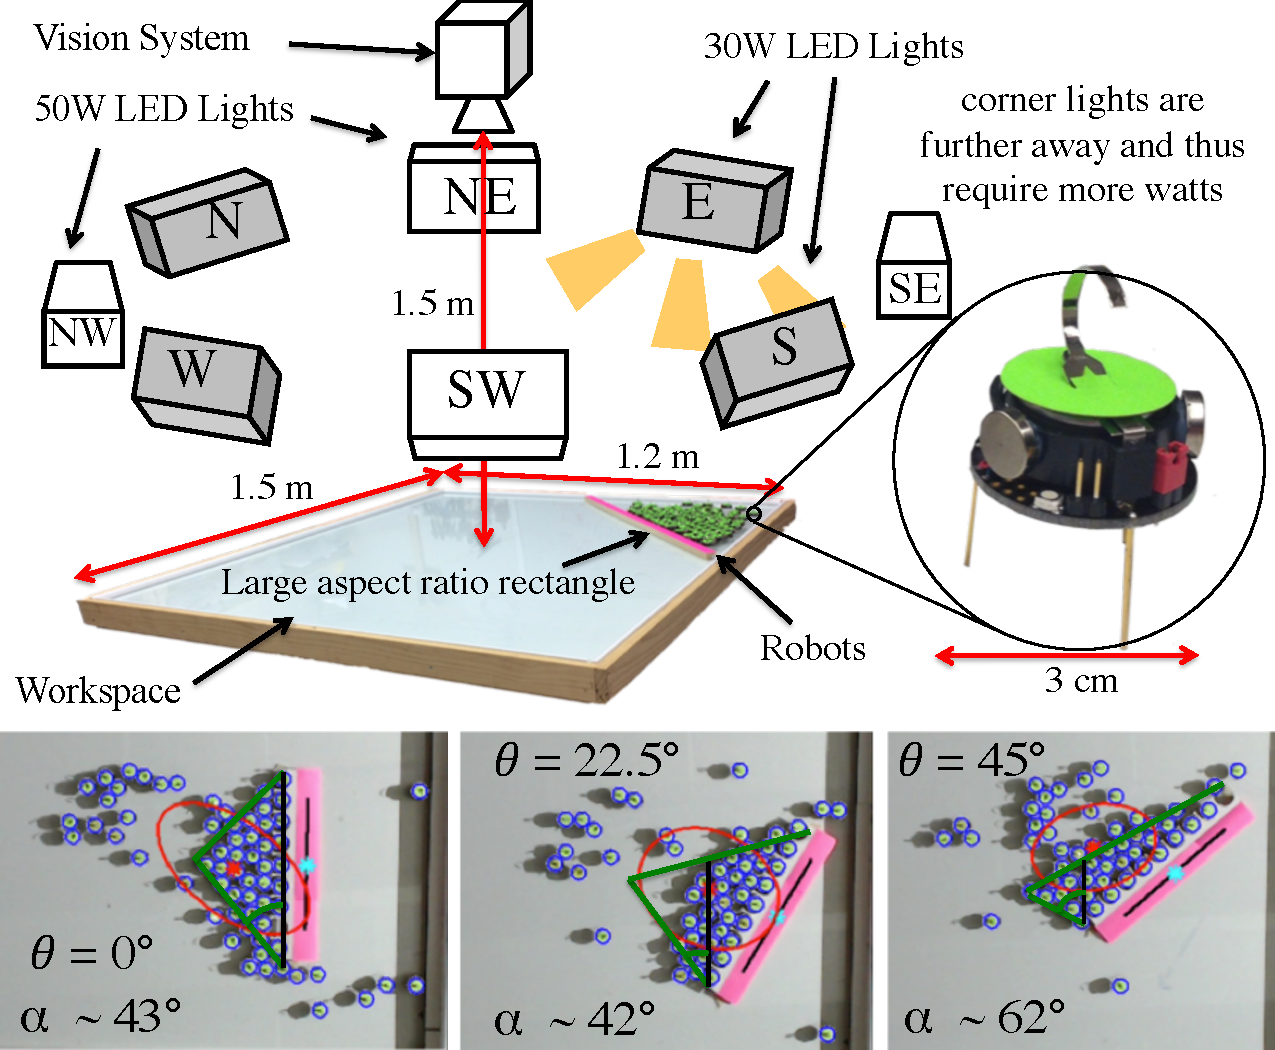
\includegraphics[width=0.5\columnwidth]{SetUp.pdf}
	\begin{overpic}[width=0.5\columnwidth]{SetUp.pdf}%\put(1,75){A}
	\end{overpic}\begin{overpic}[width=0.25\columnwidth]{AllShapesR.pdf}%\put(-0,85){B}
	\end{overpic}\begin{overpic}[width=0.25\columnwidth]{PotentialExp.pdf}%\put(-0,85){C}
	\end{overpic}
\end{center}
\caption{\label{fig:setup}
Hardware platform. At right are the shapes used for hardware experiments and a visualization of the potential field. }
\end{figure*}


\paragraph{Swarm mean control (hardware experiment)}

Unlike the PD controller \eqref{eq:PDcontrolPosition}, we cannot command a force input to the kilobots.  Instead, control is given by turning on one of eight lights.  The kilobots run a phototaxis routine where they search for an orientation that aligns them with the light source, and then move with an approximately constant velocity toward this light.  In practice, because the kilobots only have one light detector, they oscillate along this orientation.  

We use the sign of \eqref{eq:PDcontrolPosition}, and choose the closest orientation among the eight light sources.
Fig.~\ref{fig:realMean} shows that this limited, discretized control still enables regulating the mean position of a swarm of 100 robots.


\begin{figure*}
\begin{center}
	\begin{overpic}[width=\columnwidth]{RealMean}\put(42,20){\emph{t}= 90 s}\put(72,20){\emph{t}= 175 s}\end{overpic}
%	\begin{overpic}[width=0.35\columnwidth]{XYMeanControl.eps}\end{overpic}
\end{center}
\vspace{-1em}
\caption{\label{fig:realMean}
Regulating average $x$ position of 100 kilobots using control law \eqref{eq:PDcontrolPosition}.
%Mean control plot with kilobots. %\todo{place a red star and a red circle at two spots on graph, put two images of the swar at right with a red star and red circle in left hand corner of these, and put a scale bar in image}
}
\end{figure*}

%\begin{figure}
%\begin{center}
%	\includegraphics[width=\columnwidth]{XYMeanControl.eps}
%\end{center}
%\caption{\label{fig:meanRobotFig}
%Mean Control experiment with kilobots.
%}
%\end{figure}

\subsection{Automated object manipulation (hardware experiment)}

The kilobots performed five successful runs of object manipulation through the obstacle maze.
Each trial used 100 kilobots. Videos of each are in the multimedia extension. Trials two-five were performed in a row with no failures in between.  For each trial, fully charged kilobots were placed in the lower left-hand of the workspace, as shown in Fig.~\ref{fig:expSnapShot}.  The moveable object was placed in the lower center of the workspace. The same controller as in the simulation, Alg.~\ref{alg:BlockPushing}, but with discretized control inputs, was coded in {\sc Matlab}.  Trials were run until the object COM entered the goal region.  The trials ran for \{24:25, 57:37, 50:00, 36:02, 45:07\} minutes.  This is a mean of 42:38 and a standard deviation of 12:51 minutes. 
A circular object completed in 52:35 minutes. 
A square object completed in 114:31 minutes. 
A triangular object completed in XX:YY minutes.

%Rules: http://www.ijrr.org/historic/MMVideoGuideLines.pdf



\begin{figure}
\centering
%\begin{overpic}[width=\columnwidth]{Snapshots.pdf}\put(6,29){\emph{t} = 3 s}\put(38,29){\emph{t} = 410 s}\put(70,29){\emph{t} = 710 s}
%\put(15,22){\emph{t} = 1374 s}\put(49,22){\emph{t} = 2185 s}\put(83,22){\emph{t} = 2703 s}
%\end{overpic}
\begin{overpic}[width=.9\columnwidth]{Snapshots.pdf}\put(6,80){\emph{t} = 3 s}\put(38,80){\emph{t} = 410 s}\put(70,80){\emph{t} = 710 s}
\put(15,8){\emph{t} = 1374 s}\put(49,8){\emph{t} = 2185 s}\put(83,8){\emph{t} = 2703 s}
\end{overpic}
\vspace{-1em}
\caption{\label{fig:expSnapShot}{Snapshots showing the object manipulation experiment with 100 kilobots under automatic control. The automatic controller classifies pink objects as obstacles and generates a policy to the goal. See the video attachment for an animation~\cite{ShivaVideo2015}}
%\vspace{-2em}
}
\end{figure}



